\section{Root matching under perturbations}\label{sec:matching}

For a nonzero polynomial $P$, denote by $\nu_P(r)$ the number of roots of
$P$ in the closed disk $\{|z|\le r\}$, counted with multiplicity.

\begin{theorem}[Root matching]\label{thm:T4}
Let $P,Q=P+G$ be nonzero complex polynomials.
Let $D_1,\ldots,D_s$ be pairwise disjoint open disks, each containing
exactly one root of $P$ counted with multiplicity.  Suppose for a fixed
$a>0$ that
\[
 |P(z)|\geq a>|G(z)|\quad(z\in\partial D_j,\ 1\leq j\leq s).
\]
Denote by $c(r)$ the number of these disks whose closures meet $\{|z|=r\}$.
Then
\begin{equation}
 |\nu_Q(r)-\nu_P(r)|\leq c(r)+(\deg P-s)+\max(0,\deg Q-\deg P). \label{eq:T4}
\end{equation}
The same assertion holds for pairwise disjoint bounded open domains
whose boundaries are finite unions of smooth Jordan curves, with
exactly one root in each domain and the same boundary domination.
\end{theorem}

\begin{proof}
The idea is to find exactly one root of $Q$ in each selected domain by
Rouch\'e's theorem, and to count the other roots crudely, using the fact
that for each polynomial the number of them in $\{|z|\le r\}$ lies between
zero and their total number.

We use Rouch\'e's theorem in the form of
\cite[Chapter~4, Section~5.2, p.~153]{Ahlfors1979}. Let $\gamma$ be a
cycle that is homologous to zero in a region $\Omega$ and has winding
number $n(\gamma,z)\in\{0,1\}$ at every point $z$ off $\gamma$, and let
$f,g$ be analytic in $\Omega$ with $|f-g|<|f|$ on $\gamma$. Then $f$ and
$g$ have equally many zeros, counted with multiplicity, in
$\{z:n(\gamma,z)=1\}$.
We take $\Omega=\mathbb C$, in which every cycle is homologous to zero,
$f=P$, $g=Q$, and $\gamma=\partial D_j$, with its outer curve oriented
counterclockwise and its inner curves, if any, clockwise.
Since $D_j$ is the set of points inside its outer curve and outside its
inner curves, and a smooth Jordan curve winds once about each point
inside it and zero times about each point outside it, with the sign of its
orientation, we have $n(\partial D_j,z)=1$ for $z\in D_j$ and
$n(\partial D_j,z)=0$ for $z\notin\overline{D_j}$.
On $\partial D_j$ we have $|f-g|=|G|<a\le|P|=|f|$ by hypothesis.
Hence $D_j$ contains as many roots of $Q$ as of $P$, that is, exactly one,
counted with multiplicity.

Since the selected domains are pairwise disjoint and each of them contains
exactly one root of $P$ and exactly one root of $Q$, exactly $s$ roots of
each polynomial lie in these domains. We call the other roots unmatched.
Their numbers are $\deg P-s$ and $\deg Q-s=\deg P-s+\deg Q-\deg P$.
If the closure of a selected domain misses $\{|z|=r\}$, then, since the
domain is connected and the complement of the circle is the union of the
disjoint open sets $\{|z|<r\}$ and $\{|z|>r\}$, it lies entirely inside or
entirely outside that circle. Its root of $P$ is therefore counted by
$\nu_P(r)$ if and only if its root of $Q$ is counted by $\nu_Q(r)$, so
that this domain does not change the count.
On the other hand, each crossing domain, that is, one whose closure meets
the circle, changes the count by at most one, since each of its two roots
adds $0$ or $1$ to its count.
Hence the total change from selected roots is at most $c(r)$.

The numbers of unmatched roots inside the circle belong to
$[0,\deg P-s]$ and $[0,\deg Q-s]$, and their difference therefore has
absolute value at most
\[
 \max(\deg P-s,\deg Q-s)=\deg P-s+\max(0,\deg Q-\deg P),
\]
by the above expression for $\deg Q-s$.
Since $\nu_Q(r)-\nu_P(r)$ is the change from selected roots plus the
difference of the unmatched counts, we obtain \eqref{eq:T4} by the triangle
inequality.
Roots on the target circle are included in the inside count,
since the disk in $\nu_P(r)$ and $\nu_Q(r)$ is closed. Each selected root is
simple, since its total multiplicity is one.
\end{proof}

\begin{remark}\label{rem:T4-degree}
If $\deg Q\geq\deg P$, the last term in \eqref{eq:T4} is the degree difference.
For arbitrary degrees the positive part is necessary. Indeed, take
$P(z)=z^2$, $Q(z)=1$, no disks, and $0<r<1$. With the signed degree
difference we would have
\[
 2\nleq2+(0-2).
\]
\end{remark}
In this example we have $s=c(r)=0$, $\nu_P(r)=2$, since the double root $0$
lies in $\{|z|\le r\}$, and $\nu_Q(r)=0$, so that $|\nu_Q(r)-\nu_P(r)|=2$,
$\deg P-s=2$ and $\deg Q-\deg P=0-2$.

In the same way we can compare the root counts of $P$ and $Q$ in two
different disks.

\begin{corollary}[Matching across two radii]\label{cor:T4-two-radii}
Let $P$, $Q=P+G$ and the domains $D_1,\ldots,D_s$ satisfy the hypotheses of
Theorem~\ref{thm:T4}, in either of its forms. Let
$r,r'>0$, and denote by $c(r,r')$ the number of these domains whose
closures meet the closed annulus
$\{\min(r,r')\le|z|\le\max(r,r')\}$. Then
\[
 |\nu_Q(r')-\nu_P(r)|\leq c(r,r')+(\deg P-s)+\max(0,\deg Q-\deg P).
\]
\end{corollary}

\begin{proof}
Each domain $D_j$ contains exactly one root of $P$, by hypothesis, and
exactly one root of $Q$, by Rouch\'e's theorem on $\partial D_j$, applied
as in the proof of Theorem~\ref{thm:T4}, where $|G|<a\le|P|$. That step
does not involve the circle, so that only the counting changes. As
before, we call the remaining $\deg P-s$ roots of $P$ and $\deg Q-s$ roots
of $Q$ unmatched.
Let $A$ be the closed annulus between the two circles.
A domain $D_j$ whose closure misses $A$ lies in $\{|z|<\min(r,r')\}$ or in
$\{|z|>\max(r,r')\}$, since it is connected and the complement of $A$ is
the union of these two disjoint open sets. In the first case its root of
$P$ is counted by $\nu_P(r)$ and its root of $Q$ by $\nu_Q(r')$, and in
the second case neither is counted, so that the domain contributes the
same amount to $\nu_Q(r')$ and to $\nu_P(r)$. On the other hand, each of
the $c(r,r')$ remaining domains changes the difference by at most one,
since each of its two roots adds $0$ or $1$ to its count.
The numbers of unmatched roots counted by $\nu_P(r)$ and by $\nu_Q(r')$
belong to $[0,\deg P-s]$ and $[0,\deg Q-s]$, so that, as in the proof of
Theorem~\ref{thm:T4}, their difference has absolute value at most
$\deg P-s+\max(0,\deg Q-\deg P)$.
Since $\nu_Q(r')-\nu_P(r)$ is the sum of the two contributions, the
corollary follows from the triangle inequality by adding their bounds.
For $r=r'$ the annulus is the circle $\{|z|=r\}$, so that $c(r,r)=c(r)$,
and the bound reduces to \eqref{eq:T4}.
\end{proof}

\begin{lemma}[Disjoint sublevel domains near regular roots]
\label{lem:isolation-interface}
Let $a>0$ and let $\alpha$ be a root of a nonconstant polynomial $P$, with
$|P'(\alpha)|\geq d_0>0$.  Suppose
$|P''|\leq M_2$ throughout the closed disk of radius $2a/d_0$
around $\alpha$, and $4M_2a\leq d_0^2$.  Then
\[
 |P|\geq3a/2\quad\hbox{on }|z-\alpha|=2a/d_0,
\]
that disk contains exactly one root, and the component of
$\{|P|<a\}$ containing $\alpha$ lies inside it.
For any finite family of such roots with a common $a$, one can
choose a common level $b\in(a,3a/2)$ for which the corresponding
components of $\{|P|<b\}$ are pairwise disjoint bounded smooth
domains, each with exactly one root.  They satisfy the hypotheses of Theorem~\ref{thm:T4} whenever
$|G|<a$ on their closures.
\end{lemma}

\begin{proof}
The idea is to compare $P$ on the circle $|z-\alpha|=2a/d_0$ with its
linear part $P'(\alpha)(z-\alpha)$ at $\alpha$, using Taylor's theorem for
the lower bound on the circle and Rouch\'e's theorem for the single root
in the disk. For a family of roots we then choose a regular level $b$
between $a$ and $3a/2$, and the lower bound keeps each selected component
of $\{|P|<b\}$ inside the disk of its root.

Let $|z-\alpha|\le2a/d_0$. Then
\begin{align*}
 &|P(z)-P'(\alpha)(z-\alpha)|
 =|P(z)-P(\alpha)-P'(\alpha)(z-\alpha)|\\
 &\qquad=|z-\alpha|^2\Bigl|\int_0^1(1-u)P''(\alpha+u(z-\alpha))\dd u\Bigr|\\
 &\qquad\le M_2|z-\alpha|^2\int_0^1(1-u)\dd u
 =\frac{M_2}2|z-\alpha|^2,
\end{align*}
where the second equality is Taylor's theorem with integral remainder for
the function $u\mapsto P(\alpha+u(z-\alpha))$ on $[0,1]$, and the
inequality holds since $|P''|\le M_2$ on the segment from $\alpha$ to $z$,
which lies in the closed disk of radius $2a/d_0$ around $\alpha$.
For $|z-\alpha|=2a/d_0$, we therefore have
\begin{align*}
 |P(z)|&\geq|P'(\alpha)(z-\alpha)|-|P(z)-P'(\alpha)(z-\alpha)|
 \geq|P'(\alpha)||z-\alpha|-\frac{M_2}2|z-\alpha|^2\\
 &\geq d_0\cdot\frac{2a}{d_0}-\frac{M_2(2a/d_0)^2}2
 =2a-\frac{2M_2a^2}{d_0^2}
 \geq2a-\frac a2
 =\frac{3a}2,
\end{align*}
where the third inequality uses $|P'(\alpha)|\ge d_0$, and the last is the
hypothesis $4M_2a\le d_0^2$ multiplied by $a/(2d_0^2)$.

On the same circle, as in the chain above, we also have
\begin{align*}
 &|P(z)-P'(\alpha)(z-\alpha)|
 \le\frac{M_2}2|z-\alpha|^2
 =\frac{M_2(2a/d_0)^2}2
 =\frac{2M_2a^2}{d_0^2}
 \le\frac a2\\
 &\qquad<2a
 =d_0\cdot\frac{2a}{d_0}
 \le|P'(\alpha)||z-\alpha|
 =|P'(\alpha)(z-\alpha)|.
\end{align*}
Thus $f=P'(\alpha)(z-\alpha)$ and $g=P$ satisfy $|f-g|<|f|$ on the
circle. Rouch\'e's theorem, in the form used in the proof of
Theorem~\ref{thm:T4}, with $\Omega=\mathbb C$ and $\gamma$ the
counterclockwise circle, which winds once about each point of the open
disk and zero times about each point outside the closed disk, therefore
shows that $P$ has as many roots in the disk $|z-\alpha|<2a/d_0$ as the
linear polynomial $P'(\alpha)(z-\alpha)$, counted with multiplicity.
This linear polynomial is nonzero, since $|P'(\alpha)|\ge d_0>0$, and its
only root $\alpha$ lies in the disk.
Hence the open disk contains exactly one root,
and so does the closed disk, since $|P|\ge3a/2>0$ on the circle.
Since $|P|\ge3a/2>a$ on the boundary circle, the component of $\{|P|<a\}$
containing $\alpha$ does not meet this circle, and it therefore lies inside
the disk, since any connected set meeting both the interior and the
exterior of the disk meets its boundary.

For a finite family of roots, it suffices that the common level $b$
satisfies $b<3a/2$, so that the lower bound $|P|\ge3a/2$ on the circles
keeps the components inside the disks, and $b>a$, so that $|P|=b>a>|G|$ on
their boundaries. It must also avoid the values of $|P|$ at the zeros of
$P'$, so that the level $\{|P|=b\}$ is regular. We therefore choose
\[
 b\in(a,3a/2)\setminus\{|P(w)|:P'(w)=0\}.
\]
The excluded set is finite, since $P$ is nonconstant and $P'$ is a nonzero
polynomial with finitely many roots, and hence there exists such a $b$.
This level is regular, since by the Cauchy--Riemann equations the gradient
of $|P|^2$, written as a complex number, is $2P\overline{P'}$, and on
$\{|P|=b\}$ we have $P\ne0$ since $b>0$, and $P'\ne0$ by the choice of $b$.
The set $\{|P|=b\}$ is also compact, since it is closed, as $|P|$ is
continuous, and bounded, as $|P(z)|\to\infty$ as $|z|\to\infty$ for the
nonconstant polynomial $P$.
By the implicit function theorem, it is a compact smooth one-dimensional
manifold, and hence a finite union of smooth circles.

Let $\alpha$ be a designated root, that is, a
root of the family. Then the component of $\{|P|<b\}$ containing $\alpha$ is
connected and does not meet the circle $|z-\alpha|=2a/d_0$, where
$|P|\ge3a/2>b$, so that it lies inside this circle.
Since the disk contains exactly one root of $P$, the component contains
exactly its designated root. In particular, two designated roots lie in
distinct components, and distinct components of $\{|P|<b\}$ are disjoint.
Each component is open, as a component of an open set, and
bounded, since it lies in a disk. Its boundary lies in $\{|P|=b\}$, since
a boundary point $z$ satisfies $|P(z)|\le b$ by continuity, and if
$|P(z)|<b$, then a small disk about $z$ lies in $\{|P|<b\}$ and meets the
component, hence lies in it, which is impossible. Near each point of the
regular level $\{|P|=b\}$, the implicit function theorem shows that
$\{|P|<b\}$ is one side of the level curve. If the point lies on the
boundary of the component, then this side meets the component and, being
connected, lies in it, so that the nearby points of the curve lie on the
boundary as well. Consequently, the boundary of the component meets each of
the smooth circles above in an open and closed subset, and it is a union of
some of these circles.
These components are therefore disjoint bounded smooth domains, with
$|P|=b>a>|G|$ on their boundaries, by the choice of $b$ and the hypothesis
on $G$, and each of them contains exactly one root of $P$, counted with
multiplicity, so that they satisfy the hypotheses of Theorem~\ref{thm:T4}.
This holds even
when their localization disks overlap, since their disjointness comes from
the roots they contain, not from the disks.
\end{proof}

Figure~\ref{fig:phase-portrait} shows, for one polynomial with random
signs, the level curves of $|f_N|/\sigma_N(|z|)$ at the powers of $2$
around its zeros.

\begin{figure}[t]
\centering
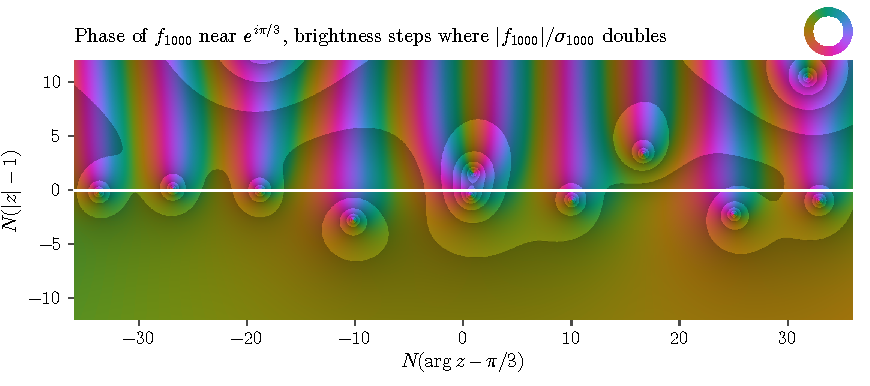
\includegraphics[width=0.85\textwidth]{figures/explanatory/phase-portrait.pdf}
\caption{Phase portrait of $f_{1000}$ near $e^{i\pi/3}$ for the sequence of
Figure~\ref{fig:root-matching}: the hue is $\arg f_{1000}$, all hues meet
at each zero, the brightness steps where $|f_{1000}|/\sigma_{1000}(|z|)$
doubles, and the white line is the unit circle. Near a zero with a large
derivative, $f_{1000}$ is nearly linear, so the small level curves are
nearly circles about it, like the boundaries of the disjoint disks about
the selected roots in Lemma~\ref{lem:isolation-interface}.}
\label{fig:phase-portrait}
\end{figure}

